\documentclass{beamer}
\usetheme{Madrid}
\usepackage[T1]{fontenc}
\usepackage{mathpazo}
\usepackage{graphicx}
\usepackage{booktabs}
\usepackage{tikz}
\usetikzlibrary{positioning,arrows.meta,shapes.geometric,fit,backgrounds,calc}
\definecolor{cetnavy}{RGB}{10,26,63}
\definecolor{cetlight}{RGB}{225,231,242}
\setbeamercolor{structure}{fg=cetnavy}
\setbeamercolor{frametitle}{bg=cetnavy,fg=white}
\setbeamercolor{title}{bg=cetnavy,fg=white}
\setbeamertemplate{navigation symbols}{}
% =====================================================================
%  EDIT YOUR DETAILS HERE — this ONE file feeds every abstract & deck.
%  (Change a value, recompile; all 36 documents update.)
% =====================================================================
\newcommand{\seminarName}{Aflah Muhammed P}      % <-- your full name (guessed from your email; please verify)
\newcommand{\seminarRoll}{TVE00CS000}            % <-- your university register/roll number
\newcommand{\seminarClassRoll}{00}               % <-- your class roll no (the short one)
\newcommand{\seminarGuide}{Prof.\ <Guide Name>}  % <-- your guide
\newcommand{\seminarDept}{Department of Computer Science and Engineering}
\newcommand{\seminarCollege}{College of Engineering Trivandrum}
\newcommand{\seminarShortCollege}{CET}           % shown in the slide footer, e.g. "Aflah Muhammed P (CET)"
\newcommand{\seminarShortTitle}{B.Tech Seminar}  % middle of the slide footer
\newcommand{\seminarDate}{July 31, 2026}
% ---------------------------------------------------------------------
% Optional: put a logo image named  cet_logo.png  in this folder and it
% will appear on every title slide automatically. If absent, it is skipped.
% =====================================================================

\title[\seminarShortTitle]{Building Rigorous Agentic Benchmarks}
\author[\seminarName\ (\seminarShortCollege)]{\seminarName \\ \seminarRoll \\ Roll No: \seminarClassRoll \\ Guide: \seminarGuide}
\institute[\seminarShortCollege]{\seminarDept \\ \seminarCollege}
\date{\seminarDate}
\titlegraphic{\IfFileExists{cet_logo.png}{\includegraphics[height=1.1cm]{cet_logo.png}}{}}
\begin{document}
\begin{frame}\titlepage\end{frame}
\begin{frame}{Table of Contents}\tableofcontents\end{frame}
\section{Introduction}
\begin{frame}{What Are Agentic Benchmarks?}
\textbf{\textit{From answering to acting}}
\begin{itemize}
\item LLM agents now write code, browse, and exploit systems.
\item Benchmarks couple environment, agent, and automated grader.
\item Leaderboard scores drive research and safety claims.
\item But a benchmark is only as good as its validity.
\end{itemize}
\end{frame}

\begin{frame}{Why Rigour Matters}
\begin{itemize}
\item Agentic tasks are multi-step and open-ended.
\item Grading is automated, not human-checked.
\item A single flaw can silently inflate scores.
\item This paper audits and fixes such flaws.
\end{itemize}
\end{frame}

\section{Literature Survey}
\begin{frame}{Prior Agentic Benchmarks}
\begin{itemize}
\item \textbf{SWE-bench Verified}: resolve real GitHub issues.
\item \textbf{TAU-bench}: tool-use in customer-service dialogues.
\item \textbf{WebArena / OSWorld}: web and desktop navigation.
\item \textbf{Cybench / CVE-Bench}: cybersecurity exploitation.
\item \textbf{KernelBench, MLE-Bench, GAIA}: code and reasoning.
\end{itemize}
\end{frame}

\begin{frame}{The Gap in Prior Work}
\begin{itemize}
\item Benchmarks published without validity audits.
\item No shared standard for grader correctness.
\item Reported numbers rarely disclose known flaws.
\item ABC fills this methodological gap.
\end{itemize}
\end{frame}

\section{Motivation}
\begin{frame}{Scores Can Mislead}
\begin{itemize}
\item Trivial agents pass tasks they should fail.
\item Graders reward empty or wrong answers.
\item Flaws distort performance up to 100\% relative.
\item Capability claims may reflect artefacts, not skill.
\end{itemize}
\end{frame}

\section{Problem Statement}
\begin{frame}{The Core Problem}
\begin{itemize}
\item How do we know a benchmark measures real ability?
\item Two threats: invalid tasks and invalid outcomes.
\item \textbf{Task validity}: solvable iff agent has the skill.
\item \textbf{Outcome validity}: grader correctly decides success.
\end{itemize}
\end{frame}

\section{Objectives}
\begin{frame}{Goals of the Paper}
\begin{itemize}
\item Audit ten widely used agentic benchmarks.
\item Formalise task validity and outcome validity.
\item Deliver an actionable checklist (ABC).
\item Quantify and correct benchmark overestimation.
\end{itemize}
\end{frame}

\section{Methodology Overview}
\begin{frame}{The ABC Pipeline}
\begin{center}
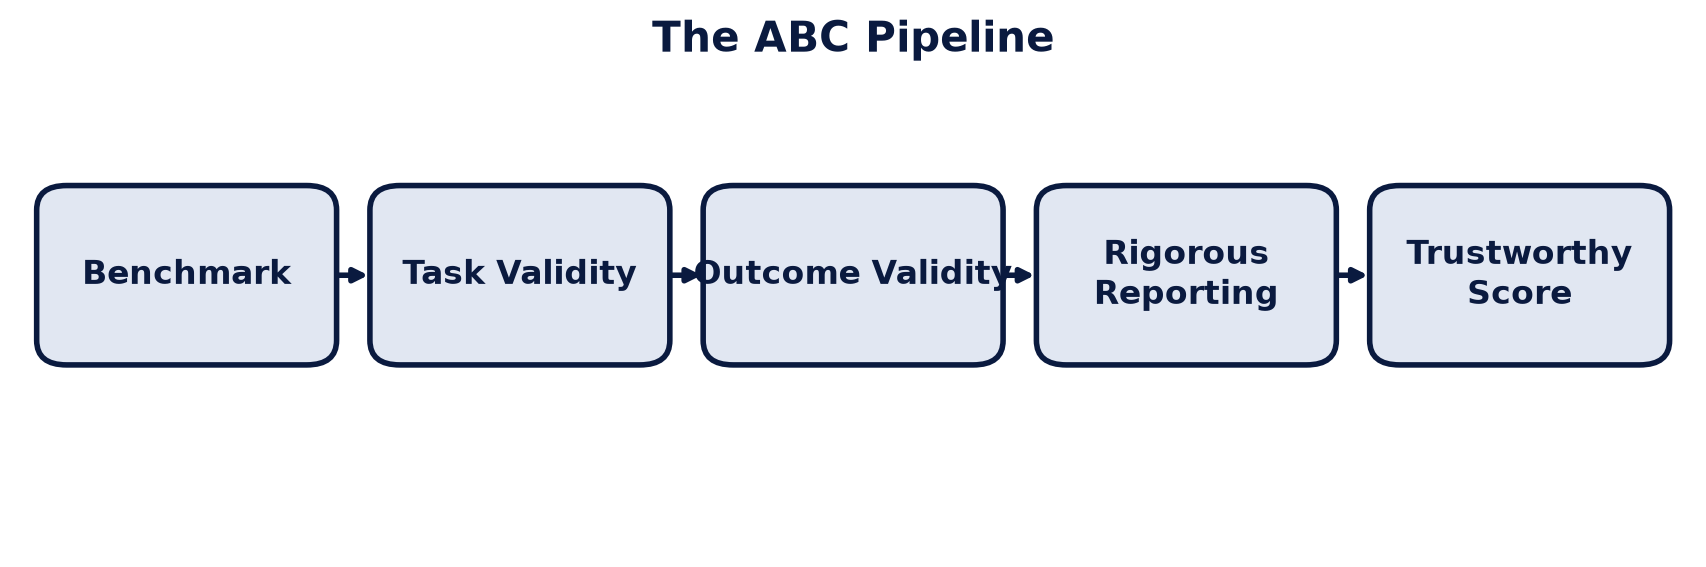
\includegraphics[width=0.9\textwidth,height=0.62\textheight,keepaspectratio]{images/rigorousbench_1.png}
\end{center}
\begin{itemize}
\item Each stage carries concrete, actionable checks.
\item Reporting handles flaws that cannot be removed.
\end{itemize}
\end{frame}

\section{System Architecture}
\begin{frame}{Anatomy of a Benchmark}
\begin{center}
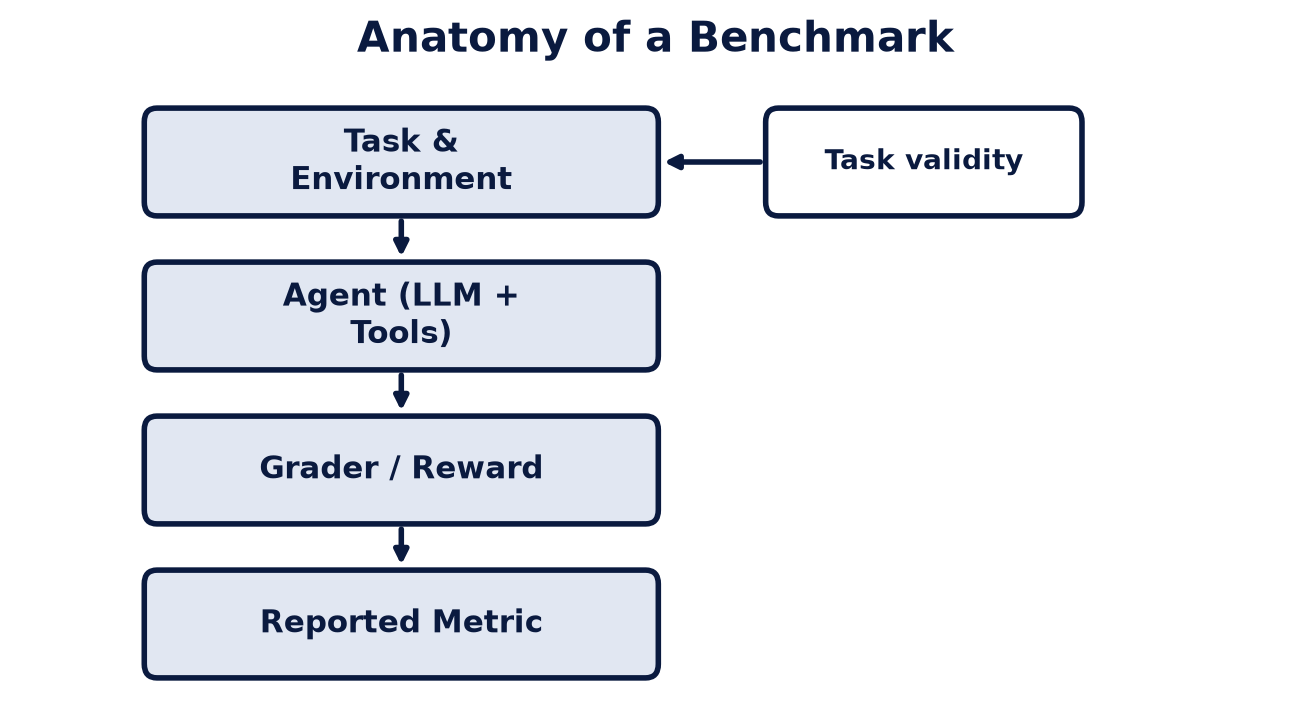
\includegraphics[width=0.9\textwidth,height=0.62\textheight,keepaspectratio]{images/rigorousbench_2.png}
\end{center}
\begin{itemize}
\item Task validity targets setup; outcome validity targets grading.
\end{itemize}
\end{frame}

\section{Data Collection}
\begin{frame}{Benchmarks Audited}
\begin{itemize}
\item Ten popular agentic benchmarks examined in depth.
\item Coverage: coding, web, OS, and cybersecurity.
\item Seven show outcome-validity flaws.
\item Seven show task-validity flaws; all lack full reporting.
\end{itemize}
\end{frame}

\section{Model Development}
\begin{frame}{The Two Validity Failure Modes}
\begin{center}
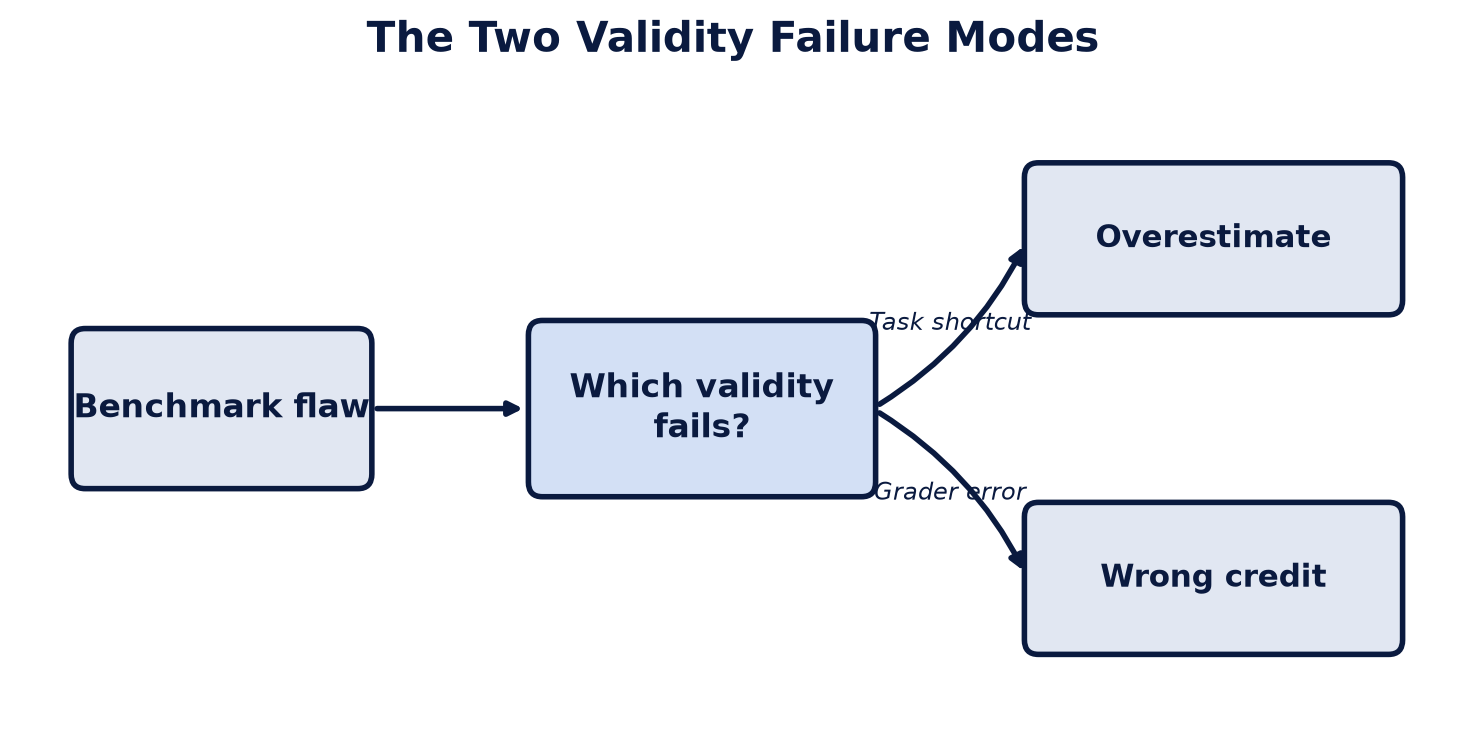
\includegraphics[width=0.9\textwidth,height=0.62\textheight,keepaspectratio]{images/rigorousbench_3.png}
\end{center}
\begin{itemize}
\item ABC provides fixes and statistical corrections for both.
\end{itemize}
\end{frame}

\section{Results}
\begin{frame}{Concrete Failures Found}
\begin{itemize}
\item \textbf{SWE-bench Verified}: weak test suites pass wrong patches.
\item \textbf{TAU-bench}: empty / no-op responses scored as success.
\item \textbf{KernelBench}: overestimation of about 31\%.
\item \textbf{CVE-Bench}: state-matching shortcuts credit fake exploits.
\end{itemize}
\end{frame}

\begin{frame}{CVE-Bench: Reported vs Corrected}
\begin{center}
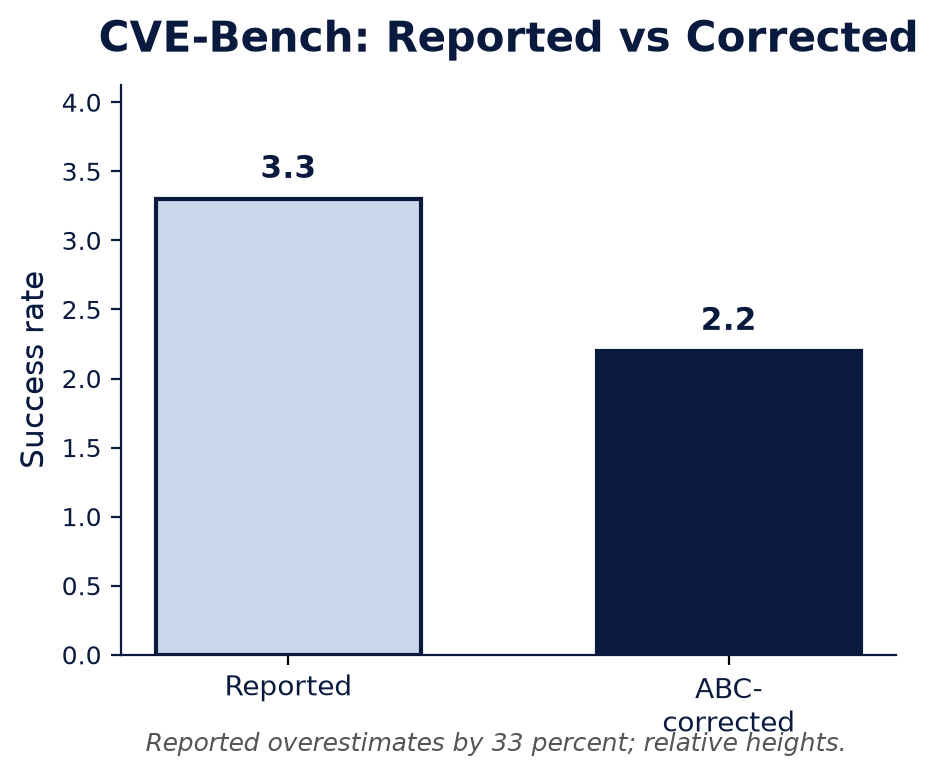
\includegraphics[width=0.9\textwidth,height=0.62\textheight,keepaspectratio]{images/rigorousbench_4.png}
\end{center}
\begin{itemize}
\item Applying ABC cut overestimation by roughly 33\%.
\item Heights are illustrative of the reported trend.
\end{itemize}
\end{frame}

\section{Discussions}
\begin{frame}{Why These Flaws Persist}
\begin{itemize}
\item Automated grading trades correctness for scale.
\item Environments leak shortcuts and stale data.
\item Outcome checks are often superficial.
\item Rigour needs deliberate, checklist-driven design.
\end{itemize}
\end{frame}

\section{Challenges}
\begin{frame}{Limitations}
\begin{itemize}
\item Perfect validity is often infeasible in practice.
\item Auditing is manual and expertise-intensive.
\item Fixes may not generalise across all benchmarks.
\item Reporting still relies on author honesty.
\end{itemize}
\end{frame}

\section{Future Work}
\begin{frame}{Directions Ahead}
\begin{itemize}
\item Automate validity checking and shortcut detection.
\item Benchmark LLM-as-a-judge graders rigorously.
\item Use frozen websites for navigation tasks.
\item Adopt ABC as a community standard.
\end{itemize}
\end{frame}

\section{Conclusion}
\begin{frame}{Takeaways}
\begin{itemize}
\item Many agentic benchmarks over- or underestimate ability.
\item Task and outcome validity are the key axes.
\item ABC gives actionable checks plus reporting norms.
\item CVE-Bench case study: overestimation cut by 33\%.
\end{itemize}
\end{frame}

\section{References}
\begin{frame}{References}
\footnotesize
\begin{itemize}
\item Y. Zhu, T. Jin, D. Kang, et al., ``Establishing Best Practices for Building Rigorous Agentic Benchmarks,'' arXiv:2507.02825, 2025.
\item C. E. Jimenez, J. Yang, et al., ``SWE-bench: Can Language Models Resolve Real-World GitHub Issues?,'' in Proc. ICLR, 2024; arXiv:2310.06770.
\item S. Zhou, F. F. Xu, et al., ``WebArena: A Realistic Web Environment for Building Autonomous Agents,'' in Proc. ICLR, 2024; arXiv:2307.13854.
\end{itemize}
\end{frame}
\begin{frame}\vfill\centering{\Huge Thank You}\vfill\end{frame}
\end{document}
